\documentclass[10pt  ,usenames, dvipsnames]{article}\usepackage[]{graphicx}\usepackage[]{color}
%% maxwidth is the original width if it is less than linewidth
%% otherwise use linewidth (to make sure the graphics do not exceed the margin)
\makeatletter
\def\maxwidth{ %
  \ifdim\Gin@nat@width>\linewidth
    \linewidth
  \else
    \Gin@nat@width
  \fi
}
\makeatother

\definecolor{fgcolor}{rgb}{0.345, 0.345, 0.345}
\newcommand{\hlnum}[1]{\textcolor[rgb]{0.686,0.059,0.569}{#1}}%
\newcommand{\hlstr}[1]{\textcolor[rgb]{0.192,0.494,0.8}{#1}}%
\newcommand{\hlcom}[1]{\textcolor[rgb]{0.678,0.584,0.686}{\textit{#1}}}%
\newcommand{\hlopt}[1]{\textcolor[rgb]{0,0,0}{#1}}%
\newcommand{\hlstd}[1]{\textcolor[rgb]{0.345,0.345,0.345}{#1}}%
\newcommand{\hlkwa}[1]{\textcolor[rgb]{0.161,0.373,0.58}{\textbf{#1}}}%
\newcommand{\hlkwb}[1]{\textcolor[rgb]{0.69,0.353,0.396}{#1}}%
\newcommand{\hlkwc}[1]{\textcolor[rgb]{0.333,0.667,0.333}{#1}}%
\newcommand{\hlkwd}[1]{\textcolor[rgb]{0.737,0.353,0.396}{\textbf{#1}}}%
\let\hlipl\hlkwb

\usepackage{framed}
\makeatletter
\newenvironment{kframe}{%
 \def\at@end@of@kframe{}%
 \ifinner\ifhmode%
  \def\at@end@of@kframe{\end{minipage}}%
  \begin{minipage}{\columnwidth}%
 \fi\fi%
 \def\FrameCommand##1{\hskip\@totalleftmargin \hskip-\fboxsep
 \colorbox{shadecolor}{##1}\hskip-\fboxsep
     % There is no \\@totalrightmargin, so:
     \hskip-\linewidth \hskip-\@totalleftmargin \hskip\columnwidth}%
 \MakeFramed {\advance\hsize-\width
   \@totalleftmargin\z@ \linewidth\hsize
   \@setminipage}}%
 {\par\unskip\endMakeFramed%
 \at@end@of@kframe}
\makeatother

\definecolor{shadecolor}{rgb}{.97, .97, .97}
\definecolor{messagecolor}{rgb}{0, 0, 0}
\definecolor{warningcolor}{rgb}{1, 0, 1}
\definecolor{errorcolor}{rgb}{1, 0, 0}
\newenvironment{knitrout}{}{} % an empty environment to be redefined in TeX

\usepackage{alltt}
\usepackage{graphicx, verbatim}
\usepackage{amsmath}
\usepackage{amssymb}
\usepackage{amscd}
\usepackage{lipsum}
\usepackage{todonotes}
\usepackage[tableposition=top]{caption}
\usepackage{ifthen}
\usepackage[utf8]{inputenc}
\usepackage{graphicx}
\usepackage{caption}
\usepackage{listings}
\usepackage{color}
\setlength{\textwidth}{6.5in} 
\setlength{\textheight}{9in}
\setlength{\oddsidemargin}{0in} 
\setlength{\evensidemargin}{0in}
\setlength{\topmargin}{-1.5cm}
\setlength{\parindent}{0cm}
\usepackage{setspace}
\usepackage{float}
\usepackage{amssymb}
\usepackage[utf8]{inputenc}
\usepackage{fancyhdr}
\usepackage{tabularx}
\usepackage{lmodern} % for bold teletype font
\usepackage{minted}
\usepackage{underscore}

\usepackage{hyperref}
\hypersetup{
  colorlinks   = true, %Colours links instead of ugly boxes
  urlcolor     = blue, %Colour for external hyperlinks
  linkcolor    = blue, %Colour of internal links
  citecolor   = red %Colour of citations
}

%\fancyhf{}
\rfoot{Andrew Tait \thepage}
\singlespacing
\usepackage[affil-it]{authblk} 
\usepackage{etoolbox}
\usepackage{lmodern}


% Notice the following package, it will help you cite papers
\usepackage[backend=bibtex ,sorting=none]{biblatex}
\bibliography{references}

\begin{filecontents*}{references.bib}

\end{filecontents*}
\IfFileExists{upquote.sty}{\usepackage{upquote}}{}
\begin{document}


\title{\LARGE Coursework  \\ Advanced Data Science (CMM536)}

\author{Andrew Tait, \textit{\href{1504693@rgu.ac.uk}{1504693@rgu.ac.uk}}}
\maketitle
% \begin{flushleft} \today \end{flushleft} 
\noindent\rule{16cm}{0.4pt}
%\underline{\hspace{3cm}
\ \\
%\thispagestyle{empty}

\section{Research}

[your text goes here]
The paper that was chosen for this work is \cite{6779381}. The authors provided a full review on different streaming algorithms and methos that handle concept drfit?. Below is a review of this paper that includes problem statement, related work and methods applied.\\

\textcolor{blue}{\textit{Notice how I cited the paper, and how does it appear in the document, to do so, you need to have a file in your working director (references.bib), this file simply contains the bibtext items for the papers you chose. These BibTex items are often avaiable to download from publishers website, see Figure~\ref{fig1}}}
\subsection{Problem Statement}
What is this paper about? your text goes here, your text goes here your text goes here your text goes here your text goes here your text goes here your text goes here

\subsection{Relevant Work}
[your text goes here your text goes here your text goes here your text goes here your text goes here your text goes here your text goes here your text goes here your text goes here your text goes here your text goes here your text goes here your text goes here your text goes here]
\subsection{Methods}
[your text goes here your text goes here your text goes here your text goes here your text goes here your text goes here your text goes here your text goes here your text goes here your text goes here your text goes here your text goes here your text goes here your text goes here]
\subsection{Results}
[your text goes here your text goes here your text goes here your text goes here your text goes here your text goes here your text goes here your text goes here your text goes here your text goes here your text goes here your text goes here your text goes here your text goes here]
\subsection{Conclusion}

[your text goes here your text goes here your text goes here your text goes here your text goes here your text goes here your text goes here your text goes here your text goes here your text goes here your text goes here your text goes here your text goes here your text goes here]




\section {Data Streams}

\subsection{Dataset Choice}

The dataset that has been chosen for this part of the coursework is the 'adult' dataset. This is avaiable on the UCI repository.

\url{https://archive.ics.uci.edu/ml/datasets/adult}

The dataset that has been chosen for this part of the course work is IRIS. This is available on the UCI repository. The set was chosen because of .... It proves to be a good set for evaluating 'x' methods .... 

\subsection{Data Exploration}

The main purpose of the adult dataset is to find out which characteristics of the us population affect if their income is either <=$50k or >=$50k



To start off I will clear the RStudio environment and import the required libaries.

\begin{knitrout}
\definecolor{shadecolor}{rgb}{0.969, 0.969, 0.969}\color{fgcolor}\begin{kframe}
\begin{alltt}
\hlcom{#Clean RStudio Environment}
\hlkwd{rm}\hlstd{(}\hlkwc{list} \hlstd{=} \hlkwd{ls}\hlstd{())}

\hlcom{#Import librarys}
\hlkwd{library}\hlstd{(caret)}
\hlkwd{library}\hlstd{(partykit)}
\hlkwd{library}\hlstd{(mlbench)}
\hlkwd{library}\hlstd{(RWeka)}
\hlkwd{library}\hlstd{(C50)}
\hlkwd{library}\hlstd{(datasets)}
\hlkwd{library}\hlstd{(rpart)}
\hlkwd{library}\hlstd{(ggplot2)}
\hlkwd{library}\hlstd{(jsonlite)}
\hlkwd{library}\hlstd{(data.table)}
\hlkwd{library}\hlstd{(RMOA)}
\hlkwd{library}\hlstd{(ROCR)}
\hlkwd{library}\hlstd{(stream)}
\hlkwd{library}\hlstd{(mlbench)}
\hlkwd{library}\hlstd{(doParallel)}
\hlkwd{require}\hlstd{(tm)}
\hlkwd{require}\hlstd{(wordcloud)}
\hlkwd{library}\hlstd{(wordcloud,}\hlkwc{quietly}\hlstd{=}\hlnum{TRUE}\hlstd{)}
\hlkwd{library}\hlstd{(RColorBrewer,}\hlkwc{quietly}\hlstd{=}\hlnum{TRUE}\hlstd{)}
\end{alltt}
\end{kframe}
\end{knitrout}



Then set the working directory to the coursework folder

\begin{knitrout}
\definecolor{shadecolor}{rgb}{0.969, 0.969, 0.969}\color{fgcolor}\begin{kframe}
\begin{alltt}
\hlcom{#Set working directory}
\hlkwd{setwd}\hlstd{(}\hlstr{"~/CMM536 Advanced Data Science/Coursework/CMM536_Coursework"}\hlstd{)}
\end{alltt}
\end{kframe}
\end{knitrout}



\clearpage

In order to the import the adult dataset, the feature names first need to be defined.
\begin{knitrout}
\definecolor{shadecolor}{rgb}{0.969, 0.969, 0.969}\color{fgcolor}\begin{kframe}
\begin{alltt}
\hlcom{#Feature names}
\hlstd{adultNames} \hlkwb{<-} \hlkwd{c}\hlstd{(}\hlstr{"age"}\hlstd{,} \hlstr{"workclass"}\hlstd{,} \hlstr{"fblwgt"}\hlstd{,}
                \hlstr{"education"}\hlstd{,} \hlstr{"education-num"}\hlstd{,}
                \hlstr{"martial-status"}\hlstd{,}
                \hlstr{"occupation"}\hlstd{,}
                \hlstr{"relationship"}\hlstd{,}
                \hlstr{"race"}\hlstd{,}
                \hlstr{"sex"}\hlstd{,}
                \hlstr{"captial-gain"}\hlstd{,}
                \hlstr{"captain-loss"}\hlstd{,}
                \hlstr{"hours-per-week"}\hlstd{,}
                \hlstr{"native-country"}\hlstd{,}
                \hlstr{"class"}\hlstd{)}
\end{alltt}
\end{kframe}
\end{knitrout}



The adult dataset is then imported from adult.data file:
\begin{knitrout}
\definecolor{shadecolor}{rgb}{0.969, 0.969, 0.969}\color{fgcolor}\begin{kframe}
\begin{alltt}
\hlcom{#Import datasets}
\hlstd{adult} \hlkwb{<-} \hlkwd{read.table}\hlstd{(}\hlstr{"data/adult.data"} \hlstd{,}\hlkwc{header} \hlstd{=} \hlnum{FALSE}\hlstd{,} \hlkwc{sep} \hlstd{=} \hlstr{","}\hlstd{,}
                         \hlkwc{strip.white} \hlstd{=} \hlnum{TRUE}\hlstd{,} \hlkwc{col.names} \hlstd{= adultNames,}
                         \hlkwc{na.strings} \hlstd{=} \hlstr{"?"}\hlstd{,} \hlkwc{stringsAsFactors} \hlstd{=} \hlnum{TRUE}\hlstd{)}
\end{alltt}
\end{kframe}
\end{knitrout}




Now the adult dataset is imported, it's time for some basic exploration

Number of rows (instances) in the dataset

\begin{knitrout}
\definecolor{shadecolor}{rgb}{0.969, 0.969, 0.969}\color{fgcolor}\begin{kframe}
\begin{alltt}
\hlkwd{nrow}\hlstd{(adult)}
\end{alltt}
\end{kframe}
\end{knitrout}

\begin{knitrout}
\definecolor{shadecolor}{rgb}{0.969, 0.969, 0.969}\color{fgcolor}\begin{kframe}
\begin{verbatim}
## [1] 32561
\end{verbatim}
\end{kframe}
\end{knitrout}

The number of columns (features)

\begin{knitrout}
\definecolor{shadecolor}{rgb}{0.969, 0.969, 0.969}\color{fgcolor}\begin{kframe}
\begin{alltt}
\hlkwd{ncol}\hlstd{(adult)}
\end{alltt}
\end{kframe}
\end{knitrout}

\begin{knitrout}
\definecolor{shadecolor}{rgb}{0.969, 0.969, 0.969}\color{fgcolor}\begin{kframe}
\begin{verbatim}
## [1] 15
\end{verbatim}
\end{kframe}
\end{knitrout}

Summary of the adult dataset:

\begin{knitrout}
\definecolor{shadecolor}{rgb}{0.969, 0.969, 0.969}\color{fgcolor}\begin{kframe}
\begin{alltt}
\hlcom{#inspect dataset}
\hlkwd{str}\hlstd{(adult)}
\end{alltt}
\end{kframe}
\end{knitrout}

\begin{knitrout}
\definecolor{shadecolor}{rgb}{0.969, 0.969, 0.969}\color{fgcolor}\begin{kframe}
\begin{verbatim}
## 'data.frame':	32561 obs. of  15 variables:
##  $ age           : int  39 50 38 53 28 37 49 52 31 42 ...
##  $ workclass     : Factor w/ 8 levels "Federal-gov",..: 7 6 4 4 4 4 4 6 4 4 ...
##  $ fblwgt        : int  77516 83311 215646 234721 338409 284582 160187 209642 45781 159449 ...
##  $ education     : Factor w/ 16 levels "10th","11th",..: 10 10 12 2 10 13 7 12 13 10 ...
##  $ education.num : int  13 13 9 7 13 14 5 9 14 13 ...
##  $ martial.status: Factor w/ 7 levels "Divorced","Married-AF-spouse",..: 5 3 1 3 3 3 4 3 5 3 ...
##  $ occupation    : Factor w/ 14 levels "Adm-clerical",..: 1 4 6 6 10 4 8 4 10 4 ...
##  $ relationship  : Factor w/ 6 levels "Husband","Not-in-family",..: 2 1 2 1 6 6 2 1 2 1 ...
##  $ race          : Factor w/ 5 levels "Amer-Indian-Eskimo",..: 5 5 5 3 3 5 3 5 5 5 ...
##  $ sex           : Factor w/ 2 levels "Female","Male": 2 2 2 2 1 1 1 2 1 2 ...
##  $ captial.gain  : int  2174 0 0 0 0 0 0 0 14084 5178 ...
##  $ captain.loss  : int  0 0 0 0 0 0 0 0 0 0 ...
##  $ hours.per.week: int  40 13 40 40 40 40 16 45 50 40 ...
##  $ native.country: Factor w/ 41 levels "Cambodia","Canada",..: 39 39 39 39 5 39 23 39 39 39 ...
##  $ class         : Factor w/ 2 levels "<=50K",">50K": 1 1 1 1 1 1 1 2 2 2 ...
\end{verbatim}
\end{kframe}
\end{knitrout}



Now that some basic data exploration is covered, next to inspect the dataset a bit further. Starting with the class distribution in the adult dataset, see (Figure~\ref{fig1})

\begin{knitrout}
\definecolor{shadecolor}{rgb}{0.969, 0.969, 0.969}\color{fgcolor}\begin{kframe}
\begin{alltt}
\hlcom{#Class Distribution}
\hlkwd{barplot}\hlstd{(}\hlkwd{table}\hlstd{(adult}\hlopt{$}\hlstd{class))}
\end{alltt}
\end{kframe}
\end{knitrout}

\begin{figure}[H]
\begin{center}
\begin{knitrout}
\definecolor{shadecolor}{rgb}{0.969, 0.969, 0.969}\color{fgcolor}
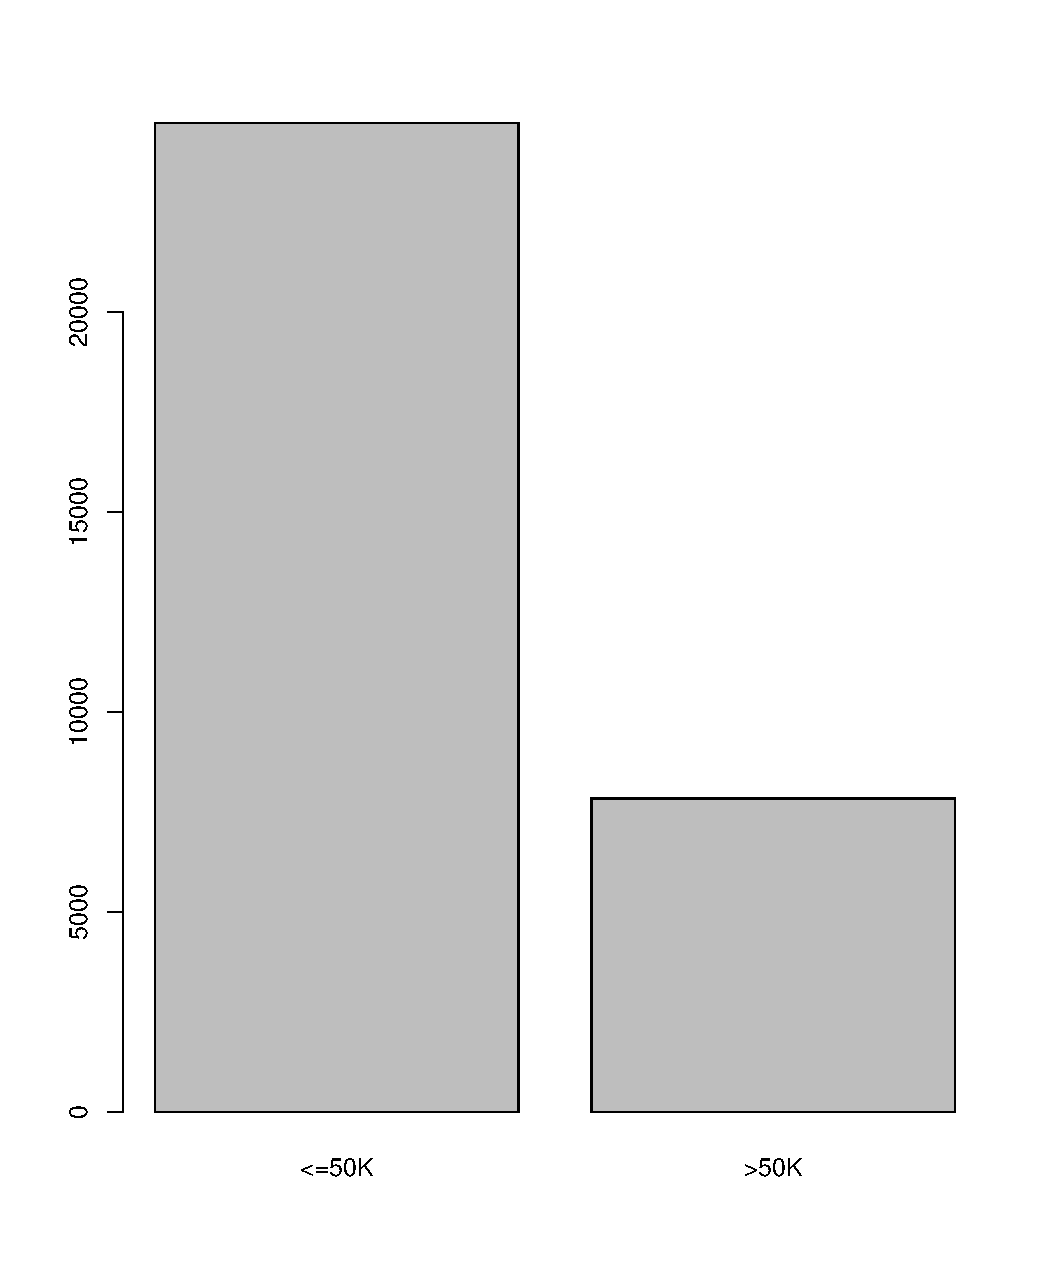
\includegraphics[width=.76\linewidth]{figure/unnamed-chunk-16-1} 

\end{knitrout}
\caption {Barplot of Class Distribution}
\label{fig1}
\end {center}
\end {figure}


\clearpage

\subsection{Build Classifier}

\subsubsection{Pre-Processing}
Before the adult dataset can classified, some pre-processing is required first.

The dataset is checked for missing values ('?')
\begin{knitrout}
\definecolor{shadecolor}{rgb}{0.969, 0.969, 0.969}\color{fgcolor}\begin{kframe}
\begin{alltt}
\hlcom{#Check for missing values ('?')}
\hlkwd{table}\hlstd{(}\hlkwd{complete.cases} \hlstd{(adult))}
\end{alltt}
\end{kframe}
\end{knitrout}

\begin{knitrout}
\definecolor{shadecolor}{rgb}{0.969, 0.969, 0.969}\color{fgcolor}\begin{kframe}
\begin{verbatim}
## 
## FALSE  TRUE 
##  2399 30162
\end{verbatim}
\end{kframe}
\end{knitrout}

As shown above there are missing values in the workclass,occupation and class columns. so these are removed.

\begin{knitrout}
\definecolor{shadecolor}{rgb}{0.969, 0.969, 0.969}\color{fgcolor}\begin{kframe}
\begin{alltt}
\hlstd{cleanadult} \hlkwb{=} \hlstd{adult[}\hlopt{!}\hlkwd{is.na}\hlstd{(adult}\hlopt{$}\hlstd{workclass)}\hlopt{& !}\hlkwd{is.na}\hlstd{(adult}\hlopt{$}\hlstd{occupation)} \hlopt{& !}\hlkwd{is.na}\hlstd{(adult}\hlopt{$}\hlstd{class),]}
\end{alltt}
\end{kframe}
\end{knitrout}




The flwgt feature is also removed as it's not required.

\begin{knitrout}
\definecolor{shadecolor}{rgb}{0.969, 0.969, 0.969}\color{fgcolor}\begin{kframe}
\begin{alltt}
\hlcom{#Remove flwgt feature}
\hlstd{cleanadult}\hlopt{$}\hlstd{fblwgt} \hlkwb{=} \hlkwa{NULL}
\end{alltt}
\end{kframe}
\end{knitrout}



Lets inspect the cleanadult dataframe before going further:

\begin{knitrout}
\definecolor{shadecolor}{rgb}{0.969, 0.969, 0.969}\color{fgcolor}\begin{kframe}
\begin{alltt}
\hlkwd{str}\hlstd{(cleanadult)}
\end{alltt}
\end{kframe}
\end{knitrout}

\begin{knitrout}
\definecolor{shadecolor}{rgb}{0.969, 0.969, 0.969}\color{fgcolor}\begin{kframe}
\begin{verbatim}
## 'data.frame':	30718 obs. of  14 variables:
##  $ age           : int  39 50 38 53 28 37 49 52 31 42 ...
##  $ workclass     : Factor w/ 8 levels "Federal-gov",..: 7 6 4 4 4 4 4 6 4 4 ...
##  $ education     : Factor w/ 16 levels "10th","11th",..: 10 10 12 2 10 13 7 12 13 10 ...
##  $ education.num : int  13 13 9 7 13 14 5 9 14 13 ...
##  $ martial.status: Factor w/ 7 levels "Divorced","Married-AF-spouse",..: 5 3 1 3 3 3 4 3 5 3 ...
##  $ occupation    : Factor w/ 14 levels "Adm-clerical",..: 1 4 6 6 10 4 8 4 10 4 ...
##  $ relationship  : Factor w/ 6 levels "Husband","Not-in-family",..: 2 1 2 1 6 6 2 1 2 1 ...
##  $ race          : Factor w/ 5 levels "Amer-Indian-Eskimo",..: 5 5 5 3 3 5 3 5 5 5 ...
##  $ sex           : Factor w/ 2 levels "Female","Male": 2 2 2 2 1 1 1 2 1 2 ...
##  $ captial.gain  : int  2174 0 0 0 0 0 0 0 14084 5178 ...
##  $ captain.loss  : int  0 0 0 0 0 0 0 0 0 0 ...
##  $ hours.per.week: int  40 13 40 40 40 40 16 45 50 40 ...
##  $ native.country: Factor w/ 41 levels "Cambodia","Canada",..: 39 39 39 39 5 39 23 39 39 39 ...
##  $ class         : Factor w/ 2 levels "<=50K",">50K": 1 1 1 1 1 1 1 2 2 2 ...
\end{verbatim}
\end{kframe}
\end{knitrout}


\clearpage

As the adult dataset is a mixture of factors, integers and characters, I decided that transforming the dataset into binary. This will be create features based on every possible value in the dataset.

The cleanadult dataframe is first copied and the class is removed (it's not being transforme dinto binary)

\begin{knitrout}
\definecolor{shadecolor}{rgb}{0.969, 0.969, 0.969}\color{fgcolor}\begin{kframe}
\begin{alltt}
\hlcom{#Copy dataset}
\hlstd{noClass} \hlkwb{<-}\hlstd{cleanadult}
\hlcom{#Remove class as it is not being transformed to binary}
\hlstd{noClass}\hlopt{$}\hlstd{class} \hlkwb{<-} \hlkwa{NULL}
\end{alltt}
\end{kframe}
\end{knitrout}




Then the noClass dataframe is transformed into binary

\begin{knitrout}
\definecolor{shadecolor}{rgb}{0.969, 0.969, 0.969}\color{fgcolor}\begin{kframe}
\begin{alltt}
\hlstd{binaryVars} \hlkwb{<-} \hlstd{caret}\hlopt{::}\hlkwd{dummyVars}\hlstd{(}\hlopt{~} \hlstd{.,} \hlkwc{data} \hlstd{= noClass)}
\hlstd{newAdult} \hlkwb{<-} \hlkwd{predict}\hlstd{(binaryVars,} \hlkwc{newdata} \hlstd{= noClass)}
\end{alltt}
\end{kframe}
\end{knitrout}



The class feature is then added to the binarised dataset
\begin{knitrout}
\definecolor{shadecolor}{rgb}{0.969, 0.969, 0.969}\color{fgcolor}\begin{kframe}
\begin{alltt}
\hlcom{#add class to binarised dataset}
\hlstd{binAdult} \hlkwb{<-}\hlkwd{cbind}\hlstd{(newAdult, cleanadult[}\hlnum{14}\hlstd{])}
\end{alltt}
\end{kframe}
\end{knitrout}



Any rows with NA values after being binary transformed.
\begin{knitrout}
\definecolor{shadecolor}{rgb}{0.969, 0.969, 0.969}\color{fgcolor}\begin{kframe}
\begin{alltt}
\hlcom{#remove any rows with NA values}
\hlstd{row.has.na} \hlkwb{<-} \hlkwd{apply}\hlstd{(binAdult,} \hlnum{1}\hlstd{,} \hlkwa{function}\hlstd{(}\hlkwc{x}\hlstd{)\{}\hlkwd{any}\hlstd{(}\hlkwd{is.na}\hlstd{(x))\})}
\hlkwd{sum}\hlstd{(row.has.na)}
\hlstd{binAdult} \hlkwb{<-} \hlstd{binAdult[}\hlopt{!}\hlstd{row.has.na,]}
\end{alltt}
\end{kframe}
\end{knitrout}

Number of NA rows removed.
\begin{knitrout}
\definecolor{shadecolor}{rgb}{0.969, 0.969, 0.969}\color{fgcolor}\begin{kframe}
\begin{verbatim}
## [1] 556
\end{verbatim}
\end{kframe}
\end{knitrout}

\clearpage

\subsubsection{Classification}

When it came to dividing the mushroom dataset into training and testing subsets, I decided to go with 80
percent training and 20 percent testing split as a starting point/baseline. 
Since the class distrubtion is unbalenced, I thought this split would cover the majority of cases.

\begin{knitrout}
\definecolor{shadecolor}{rgb}{0.969, 0.969, 0.969}\color{fgcolor}\begin{kframe}
\begin{alltt}
\hlcom{#split 80% training and 20% testing datasets}
\hlstd{inTrain} \hlkwb{<-} \hlkwd{createDataPartition}\hlstd{(}\hlkwc{y}\hlstd{=binAdult}\hlopt{$}\hlstd{class,} \hlkwc{p}\hlstd{=}\hlnum{0.8}\hlstd{,} \hlkwc{list}\hlstd{=}\hlnum{FALSE}\hlstd{)}

\hlcom{#Assign indexes to split the binAdult dataset into training and testing}
\hlstd{training} \hlkwb{<-} \hlstd{binAdult[inTrain,]}
\hlstd{testing} \hlkwb{<-} \hlstd{binAdult[inTrain,]}
\end{alltt}
\end{kframe}
\end{knitrout}




For the initial classifier I decided to go with the kNN Classifier as it has proven to be a good baseline in previous labs and exercises in R.
Before the classification begins, parallel processing is enabled to speed up this process.

\begin{knitrout}
\definecolor{shadecolor}{rgb}{0.969, 0.969, 0.969}\color{fgcolor}\begin{kframe}
\begin{alltt}
\hlcom{#Setup Parallel processing to speed up classification modelling}
\hlstd{cl} \hlkwb{<-} \hlkwd{makeCluster}\hlstd{(}\hlkwd{detectCores}\hlstd{(),} \hlkwc{type}\hlstd{=}\hlstr{'PSOCK'}\hlstd{)}
\hlkwd{registerDoParallel}\hlstd{(cl)}
\end{alltt}
\end{kframe}
\end{knitrout}



The train control is set to repeated-cross-validation with 10 folds and 3 repeats
\begin{knitrout}
\definecolor{shadecolor}{rgb}{0.969, 0.969, 0.969}\color{fgcolor}\begin{kframe}
\begin{alltt}
\hlstd{ctrl} \hlkwb{<-} \hlkwd{trainControl}\hlstd{(}\hlkwc{method} \hlstd{=} \hlstr{"repeatedcv"}\hlstd{,}
                     \hlkwc{repeats} \hlstd{=} \hlnum{3}\hlstd{,}
                     \hlkwc{number} \hlstd{=} \hlnum{10}\hlstd{,}
                     \hlkwc{verboseIter}\hlstd{=}\hlnum{TRUE}\hlstd{)}
\end{alltt}
\end{kframe}
\end{knitrout}



Next the seed is set to 1, in order to make the model reproducible and the kNN model is set up with the train control from above and k value set to 3.

\begin{knitrout}
\definecolor{shadecolor}{rgb}{0.969, 0.969, 0.969}\color{fgcolor}\begin{kframe}
\begin{alltt}
\hlcom{# ensure reproducibility of results by setting the seed to a known value}
\hlkwd{set.seed}\hlstd{(}\hlnum{1}\hlstd{)}
\hlcom{#use knn}
\hlstd{mod21.knn}\hlkwb{<-} \hlkwd{train}\hlstd{(class}\hlopt{~}\hlstd{.,} \hlkwc{data}\hlstd{=training,}
                  \hlkwc{method}\hlstd{=}\hlstr{"knn"}\hlstd{,} \hlkwc{tuneGrid}\hlstd{=}\hlkwd{expand.grid}\hlstd{(}\hlkwc{.k}\hlstd{=}\hlnum{3}\hlstd{),}\hlkwc{trControl}\hlstd{=ctrl)}
\end{alltt}
\end{kframe}
\end{knitrout}

\begin{knitrout}
\definecolor{shadecolor}{rgb}{0.969, 0.969, 0.969}\color{fgcolor}\begin{kframe}
\begin{verbatim}
## Aggregating results
## Fitting final model on full training set
\end{verbatim}
\end{kframe}
\end{knitrout}


\clearpage

Once the knn Model is complete, it’s time to analyse the results, first with a print of the kNNModel as shown below.
\begin{knitrout}
\definecolor{shadecolor}{rgb}{0.969, 0.969, 0.969}\color{fgcolor}\begin{kframe}
\begin{alltt}
\hlkwd{print}\hlstd{(mod21.knn)}
\end{alltt}
\end{kframe}
\end{knitrout}

\begin{knitrout}
\definecolor{shadecolor}{rgb}{0.969, 0.969, 0.969}\color{fgcolor}\begin{kframe}
\begin{verbatim}
## k-Nearest Neighbors 
## 
## 24131 samples
##   104 predictor
##     2 classes: '<=50K', '>50K' 
## 
## No pre-processing
## Resampling: Cross-Validated (10 fold, repeated 3 times) 
## Summary of sample sizes: 21717, 21718, 21719, 21718, 21718, 21718, ... 
## Resampling results:
## 
##   Accuracy   Kappa    
##   0.8371529  0.5550044
## 
## Tuning parameter 'k' was held constant at a value of 3
\end{verbatim}
\end{kframe}
\end{knitrout}

\clearpage

\subsubsection {Evalulation}

To evaluate the module, a confusion matrix is produced by predicting the against the testing (20 percent of the total dataset ) subset.

\begin{knitrout}
\definecolor{shadecolor}{rgb}{0.969, 0.969, 0.969}\color{fgcolor}\begin{kframe}
\begin{alltt}
\hlcom{#Evaluation}
\hlstd{predictkNN} \hlkwb{<-} \hlkwd{predict}\hlstd{(mod21.knn,testing)}
\hlkwd{confusionMatrix}\hlstd{(predictkNN, testing}\hlopt{$}\hlstd{class)}
\end{alltt}
\end{kframe}
\end{knitrout}


\begin{knitrout}
\definecolor{shadecolor}{rgb}{0.969, 0.969, 0.969}\color{fgcolor}\begin{kframe}
\begin{verbatim}
## Confusion Matrix and Statistics
## 
##           Reference
## Prediction <=50K  >50K
##      <=50K 17070  1504
##      >50K   1054  4503
##                                         
##                Accuracy : 0.894         
##                  95% CI : (0.89, 0.8979)
##     No Information Rate : 0.7511        
##     P-Value [Acc > NIR] : < 2.2e-16     
##                                         
##                   Kappa : 0.7092        
##  Mcnemar's Test P-Value : < 2.2e-16     
##                                         
##             Sensitivity : 0.9418        
##             Specificity : 0.7496        
##          Pos Pred Value : 0.9190        
##          Neg Pred Value : 0.8103        
##              Prevalence : 0.7511        
##          Detection Rate : 0.7074        
##    Detection Prevalence : 0.7697        
##       Balanced Accuracy : 0.8457        
##                                         
##        'Positive' Class : <=50K         
## 
\end{verbatim}
\end{kframe}
\end{knitrout}

\clearpage

\subsection{Build Stream Classifier}

Same as above. Complete this part as required by the coursework sheet. Again, be clear, visuals always helps in communicating results. Justify your choices and explain your methods. 


\clearpage

\section {Text Classification}
For this task a csv of leave/remain tweets of the brexit campaign was provided.

The was first imported:
\begin{knitrout}
\definecolor{shadecolor}{rgb}{0.969, 0.969, 0.969}\color{fgcolor}\begin{kframe}
\begin{alltt}
\hlstd{leaveRemainTweets} \hlkwb{<-} \hlkwd{read.csv}\hlstd{(}\hlstr{"data/leaveRemainTweets_CW.csv"}\hlstd{,} \hlkwc{header}\hlstd{=}\hlnum{TRUE}\hlstd{)}
\end{alltt}
\end{kframe}
\end{knitrout}

\subsection{Preprocessing}

In order to pre-process the leaveRemain tweets, I built a custom corpus function. Which can be found at (Figure~\ref{figbuildCorpus})


\clearpage

\subsection{Text Analysis}



\clearpage

\subsection{Text Classification}

Use one of the ‘R’ packages to build a classifier that classifies the tweets as leave tweet or remain tweets. 

Complete this part as required by the coursework sheet. Again, be clear, visuals always helps in communicating results. Justify your choices and explain your methods. 


\clearpage

\section{Appendix}

\subsection{Custom buildCorpus Function}
For the pre-processing in the text-classification task, I created a custom corpus function that will build a corpus of the leave/remain tweets and change the word filtering based on the optional function parameters.

\lstset{ 
  language=R,                     % the language of the code
  basicstyle=\tiny\ttfamily, % the size of the fonts that are used for the code
  stepnumber=1,                   % the step between two line-numbers. If it is 1, each line
                                  % will be numbered
  numbersep=5pt,                  % how far the line-numbers are from the code
  backgroundcolor=\color{white},  % choose the background color. You must add \usepackage{color}
  showspaces=false,               % show spaces adding particular underscores
  showstringspaces=false,         % underline spaces within strings
  showtabs=false,                 % show tabs within strings adding particular underscores
  frame=single,                   % adds a frame around the code
  rulecolor=\color{black},        % if not set, the frame-color may be changed on line-breaks within not-black text (e.g. commens (green here))
  tabsize=2,                      % sets default tabsize to 2 spaces
  captionpos=b,                   % sets the caption-position to bottom
  breaklines=true,                % sets automatic line breaking
  breakatwhitespace=false,        % sets if automatic breaks should only happen at whitespace
 keywordstyle=\color{RoyalBlue},      % keyword style
  commentstyle=\color{YellowGreen},   % comment style
  stringstyle=\color{ForestGreen}      % string literal style
} 
% 
% \label{figBuildCorpus}
% \begin{figure}[H]
% \caption {Custom buildCorpus function}
% \end {figure}
%     \begin{lstlisting}
%     #Custom Corpus Function for preprocessing  
% 
% buildCorpus <- function (tweets, wholeDataSet, wordAssocation){
%   corp <- Corpus(VectorSource(tweets$text))
%   
%   
%   corp <- tm_map(corp,
%                  content_transformer(function(x) iconv(x, to='ASCII',
%                                                        sub='byte')))
%   # remove stop words and other preprocessing
%  
%   corp <- tm_map(corp, content_transformer(tolower))
%   corp <- tm_map(corp, removeNumbers)
% 
%   toSpace = content_transformer( function(x, pattern) gsub(pattern," ",x) )
%   
%   
%   ##Tweet cleaning
%   
%   #credit to https://stackoverflow.com/a/31352005/8816204
%   corp <-tm_map(corp, toSpace, "(RT|via)((?:\\b\\W*@\\w+)+)")
%   corp <-tm_map(corp, toSpace, "@\\w+")
%   corp <-tm_map(corp, toSpace, "&amp")
%   
%   ##Remove URLS from tweets
%   corp <-tm_map(corp, toSpace, "httpsw+")
%   corp <-tm_map(corp, toSpace, "http:\\w+")
%   corp <-tm_map(corp, toSpace, "https:\\w+")
% 
%   corp <-tm_map(corp, toSpace, "[ \t]{2,}")
%   corp <-tm_map(corp, toSpace, "^\\s+|\\s+$")
%   
% 
%   # ##Remove obvious words /stopwords
%   if(missing(wholeDataSet)){
%     corp <- tm_map(corp, function(x)removeWords(x,c(stopwords("english"),"amp", "will", "‰Û_", "https", "http", "httpsdb")))
%   } else if(wholeDataSet == TRUE){
%     corp <- tm_map(corp, function(x)removeWords(x,c(stopwords("english"),"amp", "will", "‰Û_", "https", "http", "httpsdb", "eu", "brexit", "rt", "leave", "remain", "vote")))
%   }
% 
%   #remove punctuation last so urls are removed correctly
%   corp <- tm_map(corp, removePunctuation)
%   
%   if(missing(wordAssocation)){
%     tdm <- TermDocumentMatrix(corp)
%     
%     m <- as.matrix(tdm)
%     v <- sort(rowSums(m), decreasing = TRUE)
%     d <- data.frame(word = names(v), freq = v)
%     d$word <- gsub("˜", " ", d$word) ## Edit 2
%     
%     tweets <- d$word
%   }else if(wordAssocation == TRUE){
%     dtm <- DocumentTermMatrix(corp)
%   }
% }
% \end{lstlisting}

% Clear the page and starte a new page for references 

\clearpage
% The title for the reference section is called References 

\section{References}\label{pubs}

\printbibliography[heading =none]


\clearpage


\end{document}
